\documentclass[10pt]{beamer}

\usetheme{metropolis}
\usepackage{appendixnumberbeamer}

\usepackage{booktabs}
\usepackage[scale=2]{ccicons}

\usepackage{pgfplots}
\usepgfplotslibrary{dateplot}

\usepackage{xspace}

\usepackage{tikz}
    \usetikzlibrary{positioning}

%\usepackage{listings}
\usepackage{minted}

\usepackage{bm}%................................. Bold math symbols (after fonts)

\setbeamercolor{normal text}{bg=white}





\title{EML4930/EML6934: Lecture 06}
\subtitle{More advanced topics in matplotlib}
\date{October 5, 2017}
%\author{CJ}
\author{Charles Jekel}
%\titlegraphic{\includegraphics{images/avatarCropped.png}\vspace{58cm}}
%\institute{1. University of Florida\\ 2. Stellenbosch University, South Africa}

% \titlegraphic{\hfill\includegraphics[height=1.5cm]{logo.pdf}}

\begin{document}

\maketitle

\begin{frame}{Review syllabus}

\end{frame}

\begin{frame}{Any questions with Matplotlib pyplot?}

\end{frame}

\begin{frame}{Topics for today}

\begin{itemize}
\item Histograms
\item Contour plots
\item 3D scatter plot
\item 3D line plot
\item 3D surface plot
\item 2D Line through high dimensional space
\end{itemize}

\end{frame}

\begin{frame}{What is a histogram? }
	\begin{alertblock}{Histogram:}
		It's a type of bar graph used to approximate the probability distribution function of a continuous variable. You divide a sampled variable into a number of \textit{bins}, and then count the number of sample occurrences in each bin. You'll see the bins as the bar widths, and the frequency as the bar heights.
\end{alertblock}
\url{https://en.wikipedia.org/wiki/Histogram}
\end{frame}

\begin{frame}[fragile]{A number of distributions in np.random to sample from}
\url{https://docs.scipy.org/doc/numpy-1.13.0/reference/routines.random.html}

Let's draw samples from the Gumbel distribution

\begin{minted}
{python}
import numpy as np
mu = 4.0
beta = 0.2
# let's draw 1000 random samples from the Gumbel distribution
samples = np.random.gumbel(mu, beta, 1000)

\end{minted}
\end{frame}

\begin{frame}[fragile]{Let's create a histogram plot of the samples}
Take a look at the documentation: 
\url{https://matplotlib.org/api/pyplot_api.html?highlight=matplotlib%20pyplot%20hist#matplotlib.pyplot.hist}

\begin{minted}
{python}
matplotlib.pyplot.hist(x, bins=None, range=None, normed=False,
 weights=None, cumulative=False, bottom=None, histtype='bar',
 align='mid', orientation='vertical', rwidth=None, log=False,
 color=None, label=None, stacked=False, hold=None,
 data=None, **kwargs)
\end{minted}

There is a lot of options here. I'll try to mention the important ones.
\end{frame}

\begin{frame}[fragile]{Plotting a histogram of the Samples}
\begin{minted}
{python}
from matplotlib.pyplot as plt
plt.figure()
plt.hist(samples, bins=30, edgecolor='black')
plt.xlabel('sample value')
plt.ylabel('number of occurrences')
plt.show()
\end{minted}

\begin{figure}
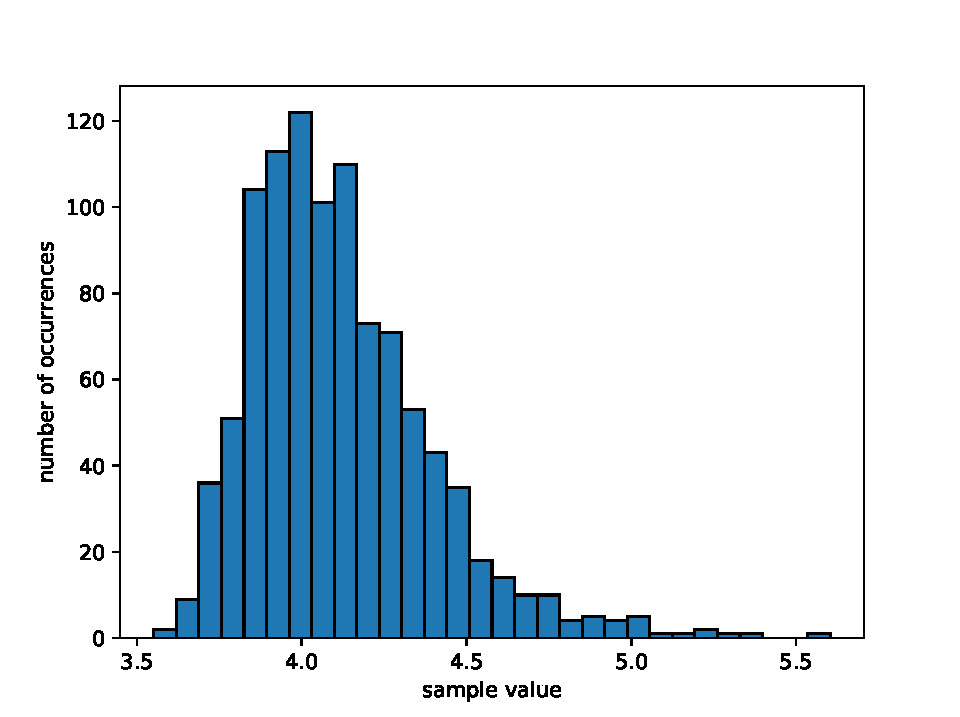
\includegraphics[width=0.6\textwidth]{figs/hist1.pdf}
\end{figure}
\end{frame}

\begin{frame}[fragile]{You generally want to work with a normalized histogram}
The integral of a probability distribution function (PDF) will be 1 by definition. The normed flag divides the frequency of each bin by the total number of samples.
\begin{minted}
{python}
plt.hist(samples, bins=30, edgecolor='black', normed=True)
\end{minted}

\begin{figure}
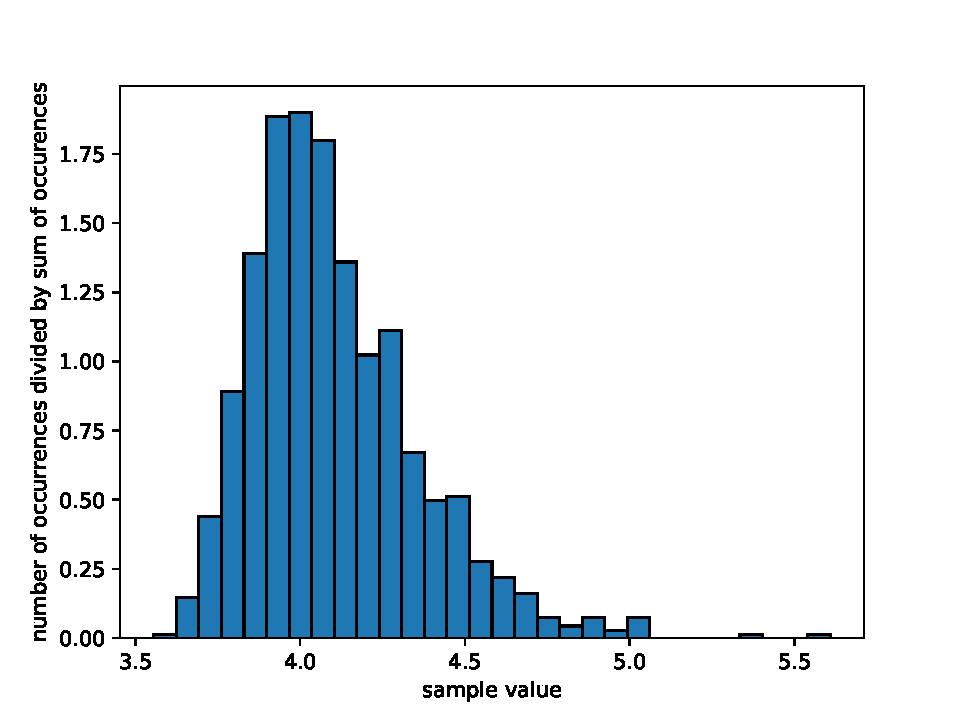
\includegraphics[width=0.6\textwidth]{figs/hist2.pdf}
\end{figure}
Note: plot created from a different random sample.
\end{frame}

\begin{frame}[fragile]{Summary of plt.hist }
\begin{itemize}
\item Histograms are sensitive to the number of bins
\item Various options to control range, bin size...
\item Use normed=True for PDFs
\item If you don't need the plot, and would work with the bins and values themselves use \mint{python}|np.histogram(a, bins=10,rane=None,Normed=False,...)|
\end{itemize}
\end{frame}

\begin{frame}[fragile]{Creating contour plots}
It's useful to represent 3D surface in a 2D plot. Generally we create contour plots to do so. 

\begin{minted}
{python}
# plot contour lines of a Function F(x,y)
plt.contour(x,y,F)

# create filled contour plot of a Function F(x,y)
plt.contourf(x,y,F)
\end{minted}

Read the documentation and examples:
\url{https://matplotlib.org/api/pyplot_api.html#matplotlib.pyplot.contour}
\url{https://matplotlib.org/api/pyplot_api.html#matplotlib.pyplot.contourf}
\end{frame}

\begin{frame}[fragile]{Let's consider the Rosenbrock function}
\begin{align*}
f(x,y) = (1 - x)^2 + 100(y-x^2)^2 \\
-1 \leq y \leq 3 \\
-2 \leq x \leq 2
\end{align*}
\begin{minted}
{python}
x = np.linspace(-2,2,100)
y = np.linspace(-1,3,100)
# we use np.meshgrid to create an x,y grid
x,y = np.meshgrid(x,y)
f = (1.0-x)**2 + (100.0*((y-(x**2))**2))
\end{minted}
\end{frame}

\begin{frame}[fragile]{Basic contour plots}
In this case we are telling the function to automatically create 100 levels
\begin{minted}
{python}
# just the lines
plt.figure()
plt.contour(x,y,f,100,
    cmap=plt.cm.viridis)
plt.colorbar()
plt.show()

# filled contour plot
plt.figure()
plt.contourf(x,y,f,100,
    cmap=plt.cm.viridis)
plt.colorbar()
plt.show()
\end{minted}
\end{frame}

\begin{frame}[fragile]{There are numerous types of color maps}
Check them all out at \url{https://matplotlib.org/users/colormaps.html}

My favorite are viridis (now default), plasma, inferno, and magma.
\begin{minted}
{python}
plt.figure()
plt.contourf(x,y,f,100,
    cmap=plt.cm.plasma)
plt.colorbar()
plt.show()

plt.figure()
plt.contourf(x,y,f,100,
    cmap=plt.cm.hot)
plt.colorbar()
plt.show()
\end{minted}
\end{frame}

\begin{frame}[fragile]{You can manually specify the levels as a list}
\begin{minted}
{python}
plt.figure()
levels=[0, 1, 5, 10, 100, 500, 1000, 2000]
plt.contourf(x,y,f,levels)
plt.colorbar()
plt.show()
\end{minted}
\end{frame}

\begin{frame}[fragile]{Contours - summary}
There are many many more features of contours. My suggestion is to read the documentation if you need to do something more advance with contours. 
\begin{figure}
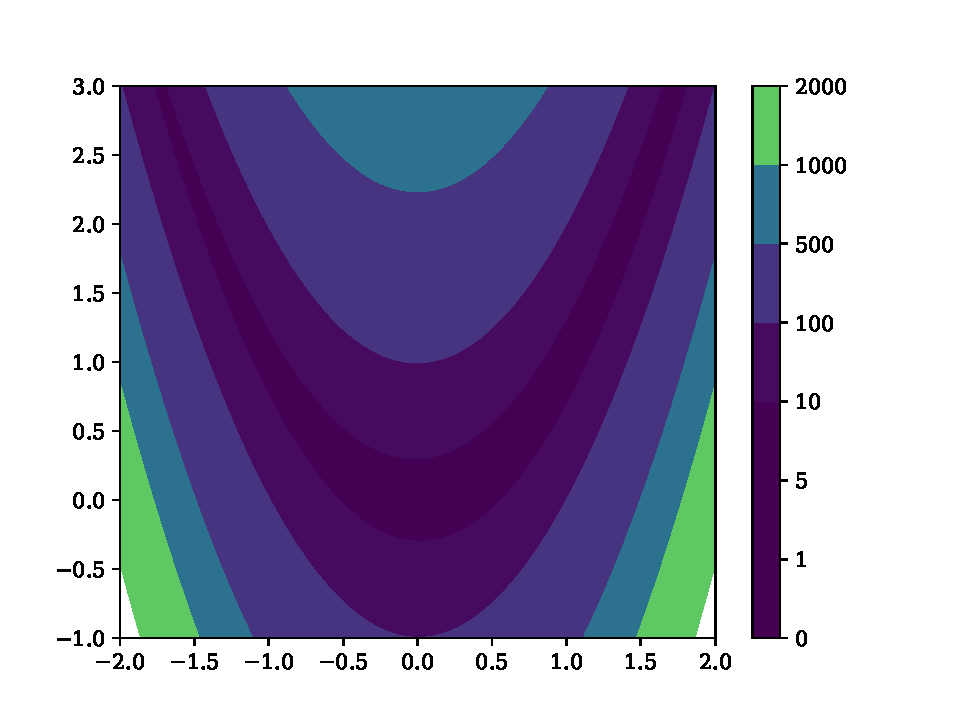
\includegraphics[width=0.6\textwidth]{figs/contours.pdf}
\end{figure}

The documentation includes a bunch of useful examples:
\url{https://matplotlib.org/api/pyplot_api.html#matplotlib.pyplot.contour}

\end{frame}

\begin{frame}[fragile]{Intro to the object orient plotting interface}
Last class we did:
\begin{minted}
{python}
import numpy as np
import matplotlib.pyplot as plt
x = np.linspace(0.0, 2.0*np.pi, 25)
plt.figure() 
plt.plot(x,np.cos(x), '--o', label='cos')
plt.plot(x,np.sin(x), '-.s', label='sin')
plt.grid(True)
plt.legend()
plt.xlabel('x axis')
plt.ylabel('y axis')

plt.show()
\end{minted}
\end{frame}

\begin{frame}[fragile]{Same result - but with OOP}
\begin{minted}
{python}
import numpy as np
import matplotlib.pyplot as plt
x = np.linspace(0.0, 2.0*np.pi, 25)

# the figure and axes of the plot are now objects
fig, ax = plt.subplots()

# you plot on the axes
ax.plot(x,np.cos(x), '--o', label='cos')
ax.plot(x,np.sin(x), '-.s', label='sin')
ax.grid(True)
ax.legend()
# However these labels are different!
ax.set_xlabel('x axis')
ax.set_ylabel('y axis')

fig.show()
\end{minted}
\end{frame}

\begin{frame}[fragile]{Alternative OOP syntax with ax.set()}
\begin{minted}
{python}
import numpy as np
import matplotlib.pyplot as plt
x = np.linspace(0.0, 2.0*np.pi, 25)
fig, ax = plt.subplots()
ax.plot(x,np.cos(x), '--o', label='cos')
ax.plot(x,np.sin(x), '-.s', label='sin')
ax.grid(True)
ax.legend()

# using set to set multiple items
ax.set(xlim=(-1,7), ylim=(-2,2), 
    xlabel='x', ylabel='y', 
    title='cos and sin plot')

fig.show()
\end{minted}
\end{frame}

\begin{frame}{Reasons to use OOP Matplotlib interface}

For the simple style of plots (like the ones covered thus far), I use the script-based interface.

For the complex plots such as
\begin{itemize}
\item subplots 
\item 3D plots
\item shapes and patches
\end{itemize}
I'll use the OOP interface.

There are basically things you can do with the OOP interface that you can't in the interface.
\end{frame}

\begin{frame}{For instance something like this}
\begin{figure}
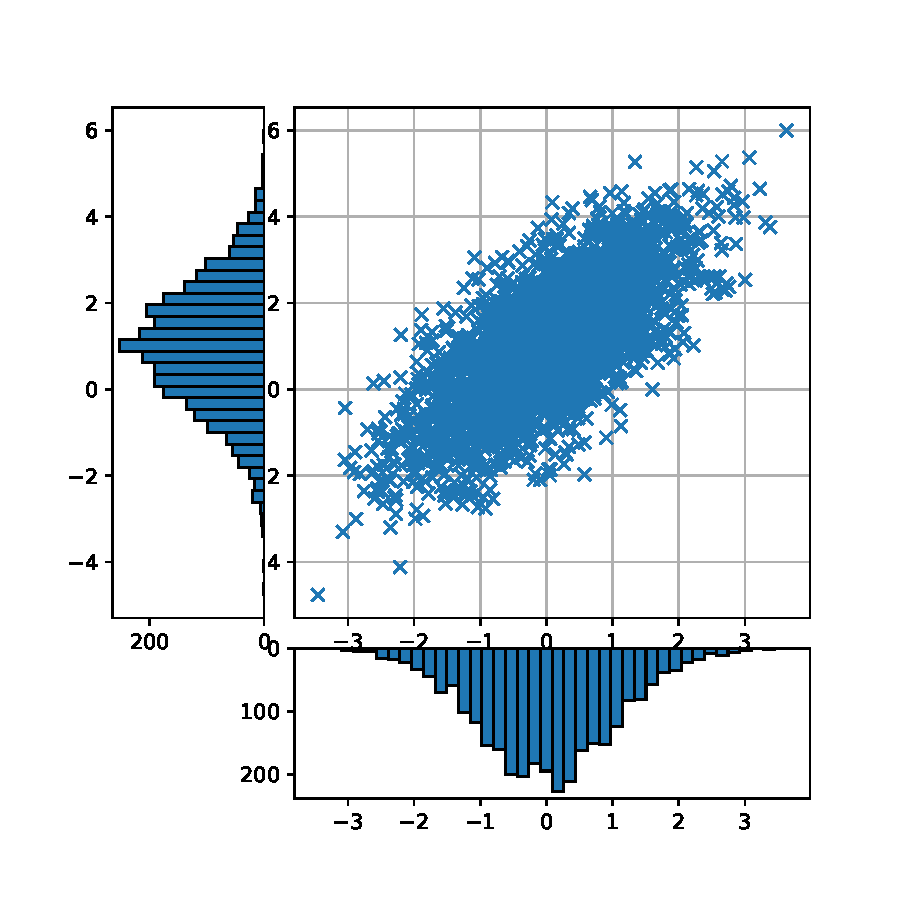
\includegraphics[width=0.8\textwidth]{figs/bivar.pdf}
\end{figure}
\end{frame}

\begin{frame}[fragile]{Code to generate 1 of 2}
\begin{minted}
{python}
# Create some normally distributed data        
mean = [0, 1]        
cov = [[1, 1], [1, 2]]        
x, y = np.random.multivariate_normal(mean, cov, 3000).T
# Set up the axes with gridspec        
fig = plt.figure(figsize=(6, 6))        
grid = plt.GridSpec(4, 4, hspace=0.2, wspace=0.2)        
main_ax = fig.add_subplot(grid[:-1, 1:])        
y_hist = fig.add_subplot(grid[:-1, 0], sharey=main_ax)        
x_hist = fig.add_subplot(grid[-1, 1:], sharex=main_ax)
        
\end{minted}
\end{frame}
\begin{frame}[fragile]{Code to generate 2 of 2}
\begin{minted}
{python}
# scatter points on the main axes        
main_ax.plot(x, y, 'x')
main_ax.grid(True)
# histogram on the attached axes        
x_hist.hist(x, 40, orientation='vertical',
 edgecolor='black')        
x_hist.invert_yaxis()
y_hist.hist(y, 40, orientation='horizontal',
 edgecolor='black')        
y_hist.invert_xaxis()
fig.show()    
\end{minted}
\end{frame}

\begin{frame}{Made with Matplotlib...}
Source code uploaded: Lectures/06/shapeDIC.py
\begin{figure}
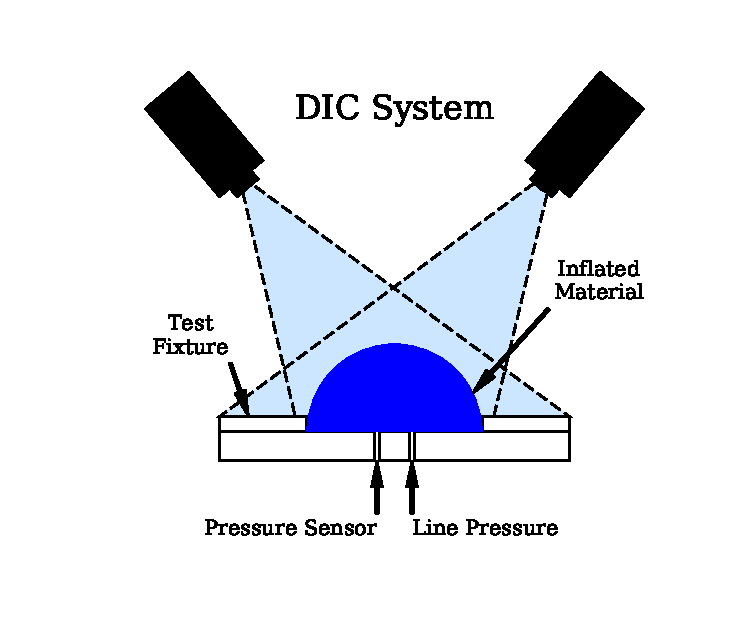
\includegraphics[width=0.9\textwidth]{figs/dicOutline.pdf}
\end{figure}
\end{frame}

\begin{frame}[fragile]{3D scatter plot in Matplotlib}
Alternative demo:
\url{https://matplotlib.org/examples/mplot3d/scatter3d_demo.html}

\begin{minted}
{python}
# we have a new import!!!    
from mpl_toolkits.mplot3d import Axes3D
fig = plt.figure()
ax = fig.add_subplot(111, projection='3d')
ax.scatter(x,y, f, 'ob')
ax.set( xlabel='X Label',
 ylabel ='Y Label', 
 zlabel='Z Label')
fig.show()

\end{minted}
\end{frame}

\begin{frame}[fragile]{3D line plot in Matplotlib}
Alternative demo:
\url{https://matplotlib.org/examples/mplot3d/lines3d_demo.html}

\begin{minted}
{python}
fig = plt.figure()
ax = fig.add_subplot(111, projection='3d')
# let's randomly choose some lines to plot in the domain
ax.plot(x[1],y[1], f[1], '-')
ax.plot(x[9],y[9], f[9], '-')
ax.plot(x[35],y[35], f[35], '-')
ax.scatter(x,y, f, 'ob')
ax.set( xlabel='X Label',
 ylabel ='Y Label', 
 zlabel='Z Label')
fig.show()
\end{minted}
\end{frame}

\begin{frame}[fragile]{3D surface plot in Matplotlib}
Alternative demo:
\url{https://matplotlib.org/examples/mplot3d/lines3d_demo.html}

\begin{minted}
{python}
fig = plt.figure()
ax = fig.add_subplot(111, projection='3d')
# let's plot the surface
# please note this only works if your x,y,z points on on a grid
# ie created with np.meshgrid !
ax.plot_surface(x,y, f)
ax.set( xlabel='X Label',
 ylabel ='Y Label',
  zlabel='Z Label')
fig.show()
\end{minted}
\end{frame}

\begin{frame}{You can do a bunch more with Matplotlib and 3D}
Please check out the 3D examples 
\url{https://matplotlib.org/mpl_toolkits/mplot3d/tutorial.html}

This concludes the basic/advance topics of Matplotlib.

\end{frame}

\begin{frame}{High dimensional visualization - line between two points}
Consider two data points 
\begin{align}
\bm{a} &= [x_1, x_2, \cdots, x_n] \\
\bm{b} &= [x_1, x_2, \cdots, x_n] \\
\end{align}
and a high dimensional function $f(x_1, x_2, \cdots, x_n)$. We can reduce this high dimensional space to a one dimensional line between the two points $\bm{a}$ and $\bm{b}$.

Consider the vector $\bm{u}$ from $\bm{a}$ to $\bm{b}$
\begin{equation}
\bm{u} = \bm{b} - \bm{a}
\end{equation}
where $\bm{u}$ indicates the direction from the point $\bm{a}$ to the point $\bm{b}$
\end{frame}

\begin{frame}{High dimensional visualization - line between two points}
We can reduce the $n$ dimensional problem into a parametric line between points $\bm{a}$ and point $\bm{b}$. The variable that will dictate the step along the line will be $\bm{r}$ such that the new high dimensional problem is represented as
\begin{align}
\bm{r} = \bm{a} + \lambda \bm{u} \\
0 \leq \lambda \leq 1
\end{align}

Remember that $\bm{r} = [x_1, x_2, \cdots, x_n]$ for some $\lambda$. To evaluate the line between $\bm{a}$ and $\bm{b}$, we evaluate
\begin{equation}
f(\bm{r})
\end{equation} 
as we vary $\lambda$ between 0 and 1. When $\lambda = 0$ we'll be at point $\bm{a}$. When $\lambda = 1$ we'll be at point $\bm{b}$.  
\end{frame}

\begin{frame}{Example: Rosenbrock function}
\begin{equation}
f(x,y) = (1 - x)^2 + 100(y-x^2)^2
\end{equation}
where 
\begin{align}
\bm{a} = [0.33, 0.57] \\
\bm{b} = [-0.11, -0.2] 
\end{align}

\textbf{Problem}: Visualize the line between $\bm{a}$ and $\bm{b}$.

\end{frame}

\begin{frame}[fragile]{Rosenbrock function visualization - between two points}
\begin{minted}
{python}
import numpy as np
import matplotlib.pyplot as plt
a = np.array([0.33, .57])
b = np.array([-0.11, -0.2])
u = b-a #
lam = np.linspace(0,1,100)
x = np.zeros(100)
y = np.zeros(100)
for i,j in enumerate(lam):
    r = (a + (j*u))
    x[i] = r[0]
    y[i] = r[1]
F = (1.0-x)**2 + (100.0*((y-(x**2))**2))
plt.figure()
plt.plot(lam,F)
plt.ylabel('F'); plt.xlabel(r'$\lambda$')
plt.show()
\end{minted}
\end{frame}

\begin{frame}{Result}
\begin{figure}
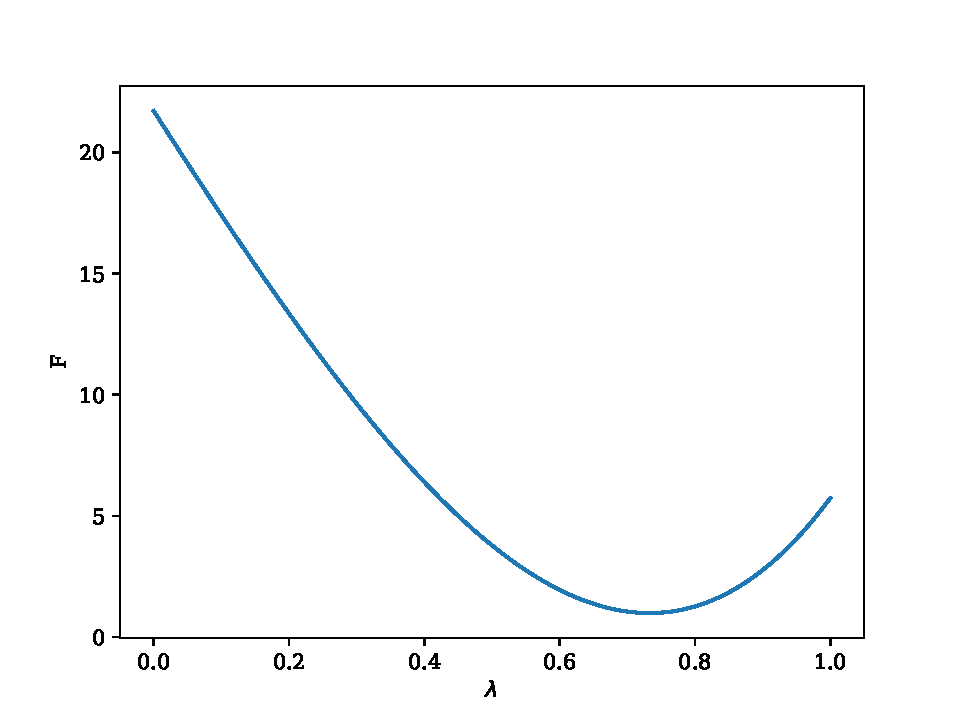
\includegraphics[width=0.9\textwidth]{figs/final.pdf}
\end{figure}
\end{frame}

%\begin{frame}{Reminder Quiz at the end of this class}
%
%\end{frame}
%
%\begin{frame}{Issues with HW?}
%
%\end{frame}
%
%\begin{frame}{What am I going to cover this lecture}
%\begin{itemize}
%\item review arrays
%\item difference between array dimensions
%\item array shaping
%\item saving and loading numpy arrays
%\item matplotlib 
%\end{itemize}
%\end{frame}
%
%\begin{frame}[fragile]{Let's consider these two arrays}
%\begin{minted}
%{python}
%import numpy as np
%a = np.array([6, 9, 2, 3, 6])
%b = np.array([[6], [9], [2], [3], [6]])
%
%# what are the dimensions
%print(a.ndim)
%print(b.ndim)
%
%# what are the shapes
%print(a.shape)
%print(b.shape)
%
%# let's print the transpose of a
%print(a)
%print(a.T)
%
%\end{minted}
%\end{frame}
%
%\begin{frame}[fragile]{Let's consider these two arrays}
%\begin{minted}
%{python}
%# let's print the transpose of b
%c = b.T
%print(b)
%print(c)
%
%# what has change?
%print(b.shape)
%print(c.shape)
%
%# what is the difference between the following?
%print(a*a)
%print(np.dot(a,a))
%\end{minted}
%\end{frame}
%
%\begin{frame}[fragile]{Saving NumPy arrays}
%\mint{python}|np.save(file, arr)|
%Save an array to a binary file in NumPy .npy format.
%\mint{python}|np.save('a_vect',a)|
%This creates a\_vect.npy file of the vector a.
%\end{frame}
%
%\begin{frame}[fragile]{Loading NumPy arrays}
%\mint{python}|np.load(file)|
%Load arrays or pickled objects from .npy, .npz or pickled files.
%\mint{python}|a_vect = np.load('a_vect.npy')|
%This loads the a\_vect.npy binary file into the a\_vect vector.
%\end{frame}
%
%\begin{frame}[fragile]{Saving NumPy arrays as plain text and loading the file}
%\mint{python}|np.savetxt(fname,X)|
%Save the array X to a text file fname.
%\mint{python}|a = numpy.loadtxt(fname)|
%Load data from a text file named fname and store this as array a.
%
%Each row in the text file must have the same number of values.
%\end{frame}
%
%\begin{frame}[fragile]{NumPy reshape}
%\begin{minted}
%{python}
%a = np.arange(6)
%b = a.reshape((3,2))
%c = a.reshape((2,3))
%d = a.reshape((6,1))
%print(b)
%print(c)
%print(d)
%
%out:
%[[0 1]
% [2 3]
% [4 5]]
%[[0 1 2]
% [3 4 5]]
%[[0 1 2 3 4 5]]
%\end{minted}
%\end{frame}
%
%\begin{frame}[fragile]{NumPy array concatenation - or joining}
%\begin{minted}
%{python}
%x = np.array([4, 5, 0, 3, 7])
%y = np.array([3, 4, 9, 7, 5])
%z = np.concatenate([x,y])
%print(z)
%
%# you can you use np.vstack to vertically stack arrays
%w = np.vstack([x,y])
%
%# you can use np.hstack to horizontally stack arrays
%v = np.hstack([w,w])
%\end{minted}
%\end{frame}
%
%\begin{frame}[fragile]{flatten any ndarray into one dimension}
%\begin{minted}
%{python}
%k = np.random.random((5,3,2,6,8))
%print(k.ndim)
%k_flat = k.flatten()
%print(k_flat.ndim)
%print(k_flat.size)
%
%out:
%5
%1
%1440
%\end{minted}
%\end{frame}
%
%\begin{frame}{matplotlib}
%Matplotlib tries to make easy things easy and hard things possible. You can generate plots, histograms, power spectra, bar charts, errorcharts, scatterplots, etc., with just a few lines of code. For a sampling, see the screenshots, thumbnail gallery, and examples directory
%
%For simple plotting the pyplot module provides a MATLAB-like interface, particularly when combined with IPython. For the power user, you have full control of line styles, font properties, axes properties, etc, via an object oriented interface or via a set of functions familiar to MATLAB users.
%
%\url{https://matplotlib.org/}
%\end{frame}
%
%\begin{frame}{For reference}
%Dr. Jake VanderPlas’s Python Data Science Handbook: Essential Tools for Working with Data.
%
%Chapter 4: Visualization with Matplotlib
%
%\url{http://nbviewer.jupyter.org/github/jakevdp/PythonDataScienceHandbook/blob/master/notebooks/Index.ipynb}
%\end{frame}
%
%\begin{frame}[fragile]{matplotlib pyplot - MATLAB like plotting framework}
%\begin{minted}
%{python}
%import numpy as np
%import matplotlib.pyplot as plt
%
%x = np.linspace(0.0, 2.0*np.pi, 25)
%
%# you can specify a figure number or string name
%# but by default plt.figure() will create a number ordered 
%# figure name Ex: plt.figure('my figure') or plt.figure(1)
%plt.figure() 
%# create a line plot by default
%plt.plot(x,np.cos(x))
%# show the plot
%plt.show()
%\end{minted}
%\end{frame}
%
%\begin{frame}{matplotlib linestyles}
%\begin{table}
%\begin{tabular}{ll}
%\textbf{Linestyle} & \textbf{Description}  \\
%\hline
%'-' or 'solid' 	 &  solid line\\
%'--' or 'dashed' &	dashed line\\
%'-.' or 'dashdot'& 	dash-dotted line\\
%':' or 'dotted'  &	dotted line\\
%'None'           &	draw nothing\\
%' '              &	draw nothing\\
%'' 	             &  draw nothing\\
%\end{tabular}
%\end{table}
%\end{frame}
%
%\begin{frame}[fragile]{Plotting cosine with a dashed line}
%\begin{minted}
%{python}
%import numpy as np
%import matplotlib.pyplot as plt
%
%x = np.linspace(0.0, 2.0*np.pi, 25)
%
%plt.figure() 
%
%# all you need to do is pass the linestyle as an attribute
%plt.plot(x,np.cos(x), '--')
%plt.show()
%\end{minted}
%\end{frame}
%
%\begin{frame}{Scatter plot markers}
%and more at - \url{https://matplotlib.org/api/markers_api.html} 
%\begin{table}
%\begin{tabular}{ll}
%\textbf{Marker} & \textbf{Description}  \\
%\hline
%"." &	point\\
%"," &	pixel\\
%"o" &	circle\\
%"v" &	triangle\_down\\
%"$<$" &	triangle\_left\\
%"$>$" &	triangle\_right\\
%"1" &	tri\_down\\
%"2" &	tri\_up\\
%"3" &	tri\_left\\
%"4" &	tri\_right\\
%"8" &	octagon\\
%"s" &	square\\
%"p" &	pentagon\\
%"P" &	plus (filled)\\
%\end{tabular}
%\end{table}
%\end{frame}
%
%\begin{frame}[fragile]{Scatter plot cosine}
%\begin{minted}
%{python}
%import numpy as np
%import matplotlib.pyplot as plt
%
%x = np.linspace(0.0, 2.0*np.pi, 25)
%
%plt.figure() 
%
%# all you need to do is pass the marker into plot
%plt.plot(x,np.cos(x), 'o')
%plt.show()
%\end{minted}
%\end{frame}
%
%\begin{frame}[fragile]{You can easily combine markers and linestyles}
%\begin{minted}
%{python}
%import numpy as np
%import matplotlib.pyplot as plt
%
%x = np.linspace(0.0, 2.0*np.pi, 25)
%
%plt.figure() 
%
%# this will plot a -- linestyle with circles at the data points
%plt.plot(x,np.cos(x), '--o')
%plt.show()
%\end{minted}
%\end{frame}
%
%\begin{frame}{basic built-in colors in matplotlib}
%and more at - \url{https://matplotlib.org/api/colors_api.html} 
%\begin{table}
%\begin{tabular}{ll}
%\textbf{Code} & \textbf{Color}  \\
%\hline
%b & blue\\
%g & green\\
%r & red\\
%c & cyan\\
%m & magenta\\
%y & yellow\\
%k & black\\
%w & white\\
%\end{tabular}
%\end{table}
%\end{frame}
%
%\begin{frame}[fragile]{You can specify the built in color into plot}
%\begin{minted}
%{python}
%import numpy as np
%import matplotlib.pyplot as plt
%
%x = np.linspace(0.0, 2.0*np.pi, 25)
%
%plt.figure() 
%
%# forcing the line and dot color to be blue
%plt.plot(x,np.cos(x), 'b--o')
%plt.show()
%\end{minted}
%\end{frame}
%
%\begin{frame}[fragile]{Alternatively use color=''}
%\begin{minted}
%{python}
%# specify color by name 
%plt.plot(x, np.cos(x), color='blue')
%
%# short color code (rgbcmyk)
%plt.plot(x, np.cos(x), color='g') 
%
%# Grayscale between 0 and 1                   
%plt.plot(x, np.cos(x), color='0.75')        
%
%# Hex code (RRGGBB from 00 to FF) 
%plt.plot(x, np.cos(x), color='#FFDD44')     
%
%# RGB tuple, values 0 and 1 
%plt.plot(x, np.cos(x), color=(1.0,0.2,0.3)) 
%
%# all HTML color names supported
%plt.plot(x, np.cos(x), color='chartreuse') 
%\end{minted}
%\end{frame}
%
%\begin{frame}[fragile]{Adjusting the plot with axes limit}
%\begin{minted}
%{python}
%import numpy as np
%import matplotlib.pyplot as plt
%
%x = np.linspace(0.0, 2.0*np.pi, 25)
%
%plt.figure() 
%plt.plot(x,np.cos(x), 'b--o')
%
%# set the x axis limit
%plt.xlim(-1,7)
%
%# set the y axis limit
%plt.ylim(-2,2)
%
%plt.show()
%\end{minted}
%\end{frame}
%
%\begin{frame}[fragile]{Adding a grid}
%\url{https://matplotlib.org/api/pyplot_api.html?highlight=matplotlib%20pyplot%20grid#matplotlib.pyplot.grid}
%
%grid(b=None, which='major', axis='both', **kwargs)
%
%    kwargs are used to set the grid line properties, e.g.,:
%    \mint{python}|ax.grid(color='r', linestyle='-', linewidth=2)|
%\begin{minted}
%{python}
%import numpy as np
%import matplotlib.pyplot as plt
%x = np.linspace(0.0, 2.0*np.pi, 25)
%plt.figure() 
%plt.plot(x,np.cos(x), 'b--o')
%# create a grid
%plt.grid(True)
%plt.show()
%\end{minted}
%\end{frame}
%
%\begin{frame}[fragile]{Labels and legend}
%\begin{minted}
%{python}
%import numpy as np
%import matplotlib.pyplot as plt
%x = np.linspace(0.0, 2.0*np.pi, 25)
%plt.figure() 
%
%# add label='my_label'
%plt.plot(x,np.cos(x), '--o', label='cos')
%plt.plot(x,np.sin(x), '-.s', label='sin')
%plt.grid(True)
%
%# add legend
%plt.legend()
%# legend automatically chooses the location
%# but you can specify the simple quadrant based location as
%# plt.legend(loc=1) puts the legend in the first quadrant
%
%plt.show()
%\end{minted}
%\end{frame}
%
%\begin{frame}[fragile]{matplotlib title and axis label}
%\begin{minted}
%{python}
%import numpy as np
%import matplotlib.pyplot as plt
%x = np.linspace(0.0, 2.0*np.pi, 25)
%plt.figure() 
%plt.plot(x,np.cos(x), '--o', label='cos')
%plt.plot(x,np.sin(x), '-.s', label='sin')
%plt.grid(True)
%plt.legend()
%# adding a title
%plt.title('Cos and sin')
%
%# x and y axis labels
%plt.xlabel('x axis')
%plt.ylabel('y axis')
%
%plt.show()
%\end{minted}
%\end{frame}
%
%\begin{frame}[fragile]{matplotlib pyplot savefig}
%\url{https://matplotlib.org/api/pyplot_api.html?highlight=matplotlib%20pyplot%20savefig#matplotlib.pyplot.savefig}
%
%\begin{minted}
%{python}
%plt.savefig(fname, dpi=None, facecolor='w', edgecolor='w',
%        orientation='portrait', papertype=None, format=None,
%        transparent=False, bbox_inches=None, pad_inches=0.1,
%        frameon=None)
%\end{minted}
%
%How I normally create publication quality pictures:
%\begin{minted}
%{python}
%plt.savefig('my_fig.pdf', dpi=600, format='pdf',
%            bbox_inches='tight')
%\end{minted}
% Most backends support png, pdf, ps, eps and svg.
%\end{frame}
%
%\begin{frame}[fragile]{saving my cosine and sin plot}
%Depending on your active Python interpreter, you'll have issues with plt.show()
%\begin{minted}
%{python}
%import numpy as np
%import matplotlib.pyplot as plt
%x = np.linspace(0.0, 2.0*np.pi, 25)
%plt.figure() 
%plt.plot(x,np.cos(x), '--o', label='cos')
%plt.plot(x,np.sin(x), '-.s', label='sin')
%plt.grid(True)
%plt.legend()
%plt.xlabel('x axis')
%plt.ylabel('y axis')
%
%plt.savefig('my_fig.pdf', dpi=600, format='pdf',
%             bbox_inches='tight')
%\end{minted}
%\end{frame}
%
%\begin{frame}{Created this plot}
%\begin{figure}
%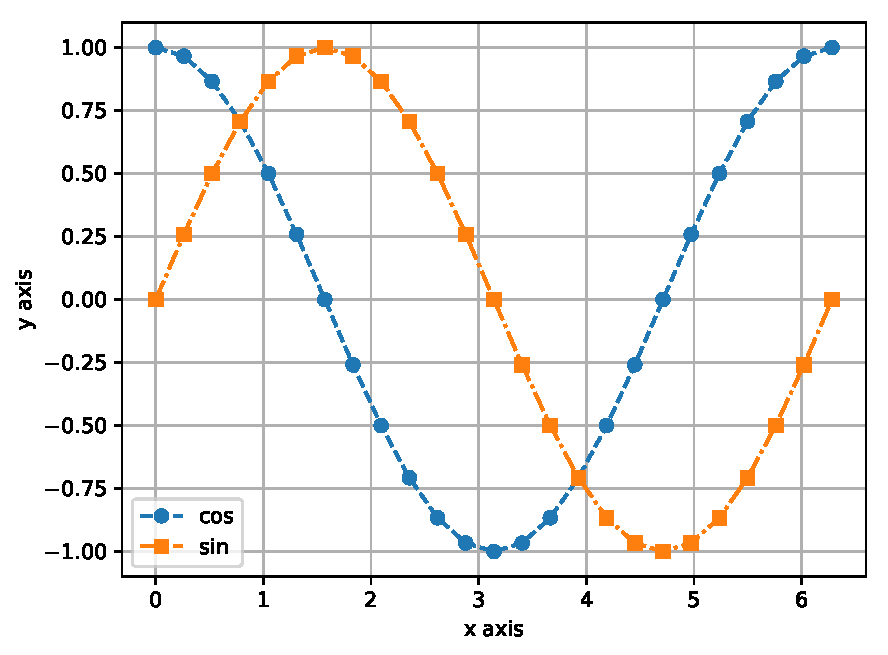
\includegraphics[width=0.9\textwidth]{fig/my_fig.pdf}
%\end{figure}
%\end{frame}


\end{document}
